% Horizon penetrating coordinates (vs. Schwarzschild coordinates)
% for a black hole spacetime, with excision
% Author: Jonah Miller
\documentclass[tikz,border=6pt]{standalone}
\usepackage{tikz}
\usepackage{ifthen}
\usepackage{calc}
\usepackage{fp}

\usetikzlibrary{arrows}
\usetikzlibrary{arrows.meta}
\usetikzlibrary{decorations.markings}
\usepackage{pgfplots}

%\tikzset{>={Latex[length=3mm]}}

\begin{document}
%\newlength{\asdf}

%\foreach \carx in {2.91,2.85,...,0.8}
%\foreach \carx in {2.91, 2.86, 2.80, 2.75, 2.69, 2.64, 2.59, 2.53, 2.48, 2.42, 2.37, 2.31, 2.26, 2.21, 2.15, 2.10, 2.04, 1.96, 1.94, 1.88, 1.83, 1.77, 1.72, 1.67, 1.61, 1.56, 1.50, 1.45, 1.40, 1.34, 1.29, 1.23, 1.18, 1.12, 1.07, 1.02, 0.96, 0.91, 0.85, 0.80}
%\foreach \carx in {2.91, 2.88, 2.86, 2.83, 2.80, 2.77, 2.74, 2.71, 2.67, 2.64, 2.60, 2.56, 2.52, 2.48, 2.43, 2.38, 2.33, 2.26, 2.19, 2.09, 1.85, 1.62, 1.52, 1.45, 1.38, 1.33, 1.28, 1.23, 1.19, 1.15, 1.11, 1.07, 1.04, 1.00, 0.97, 0.94, 0.91, 0.88, 0.85, 0.83, 0.80}
\foreach \carx in {2.91, 2.88, 2.84, 2.80, 2.77, 2.73, 2.68, 2.64, 2.59, 2.54, 2.48, 2.41, 2.33, 2.23, 1.99, 1.74, 1.64, 1.56, 1.49, 1.43, 1.38, 1.33, 1.29, 1.24, 1.20
}
{
\begin{tikzpicture}[scale=1.4]
%\def\carx{\asdf}
\def\flagheight{4/5}
\def\carlength{0.2}

\draw[] (4.05,{\flagheight + 1}) node{\hphantom{asdfasdf}};
\draw[] (2,1.5) node[red,align=center]{$r = -F^2$};
\draw[] (2,-0.9) node[]{\vphantom{asdf}};

\draw[scale=1,domain=0.3:4.05,smooth,variable=\x] plot ({\x},{\flagheight*cos(90*\x)});

\draw[-,fill=green] (4,\flagheight) -- (4,{\flagheight + 0.4}) -- (4.2,{\flagheight + 0.3}) -- (4,{\flagheight+0.2});



%\def\carx{2.71}
\def\cary{\flagheight*cos(90*\carx)}

%\def\m{\ifthenelse{\equal{\carx}{2}} {100000} {1/(\flagheight*sin(90*\carx))}}

\ifthenelse{\lengthtest{\carx pt < 2 pt}} {\def\fff{-1}} {\def\fff{1}}

\def\m{1/(\flagheight*sin(90*\carx))}
\def\mt{(\flagheight*sin(90*\carx))}
%\def\deltax{(\fff)*sqrt(0.01 / (1 + (\m)*(\m)) )}
\def\deltax{(\fff)*sqrt((0.01*\mt*\mt)/(1 + \mt*\mt))}

\ifthenelse{\lengthtest{\carx pt < 1.85 pt} \OR \lengthtest{\carx pt > 2.15 pt}}{\def\deltay{(\m) * (\deltax)}}{\def\deltay{-0.1}}
%\def\deltay{(\m) * (\deltax)}
\def\carxtwo{\carx - \deltax}
\def\carytwo{\cary - \deltay}


%\ifthenelse{\lengthtest{\carx pt < 1.5 pt} \OR \lengthtest{\carx pt > 2.5 pt}}{\def\carxx{(\carx - \carlength)}}{\def\carxx{(\carx - 2*\carlength  + 0.89*(\carx - 2)^2)}}
%\def\carxx{(\carx - \carlength + -\carlength + 0.5*(\carx - 2)^2)}
\def\carxx{\carx - sqrt((\carlength^2) / (1 + (\mt)^2))}
%\def\carxx{(\carx - \carlength - 0.15*abs(cos(90*\carx)))}
\def\caryy{\flagheight*cos(90*(\carxx))}

%\def\m{\ifthenelse{\equal{\carx}{2}} {100000} {1/(\flagheight*sin(90*\carx))}}

%\def\aaaa{0.15*abs(cos(90*\carx))}

%\setlength{\asdf}{\carx pt - \carlength pt - \aaaa pt }


\FPeval{\asdf}{(\carx - \carlength - 0.15*abs(cos(90*\carx)))}

\ifthenelse{\lengthtest{\asdf pt  < 2 pt }} {\def\ffff{-1}} {\def\ffff{1}}

\def\mm{1/(\flagheight*sin(90*(\carxx)))}
\def\mtt{(\flagheight*sin(90*(\carxx)))}

\def\deltaxx{(\ffff)*sqrt((0.01*(\mtt)*(\mtt))/(1 + (\mtt)*(\mtt)))}

\ifthenelse{\lengthtest{\asdf pt < 1.85 pt} \OR \lengthtest{\asdf pt > 2.15 pt}}{\def\deltayy{(\mm) * (\deltaxx)}}{\def\deltayy{-0.1}}
%\def\deltay{(\m) * (\deltax)}
\def\carxxtwo{\carxx - \deltaxx}
\def\caryytwo{\caryy - \deltayy}





\def\angle{atan((\carxxtwo - \carxtwo) / (\caryytwo - \carytwo)) }

\def\riix{\carxtwo - \carxxtwo}
\def\riiy{\carytwo - \caryytwo}
\def\coeffang{(((\riiy) / (\riix)))}

\def\dddeltax{(sqrt(0.05 / (1 + \coeffang^2)))}
\def\dddeltay{-((\dddeltax) * \coeffang)}

%\draw[-,fill=black,rotate around={{0}:({\carxxtwo},{\caryytwo})}] ({\carxxtwo-0.1},{\caryytwo+0.05}) rectangle({\carxxtwo + sqrt((\carxtwo - \carxxtwo)^2 + (\carytwo - \caryytwo)^2) },{\caryytwo + 0.25});
%\draw[-,fill=black,rotate around={{0}:({\carxxtwo},{\caryytwo})}] ({\carxtwo},{\carytwo}) rectangle({\carxxtwo + sqrt((\carxtwo - \carxxtwo)^2 + (\carytwo - \caryytwo)^2) },{\caryytwo + 0.25});
\draw[line width=0.3cm, black, cap=rect] ({\carxxtwo - \deltaxx}, {\caryytwo - \deltayy}) -- ({\carxtwo - \deltax}, {\carytwo - \deltay}); 


\def\deltaxnorm{sqrt((\deltaxx)^2 + (\deltayy)^2)}
\def\deltaxperpnorm{(\deltaxx)/(\deltaxnorm)}
\def\deltayperpnorm{(\deltayy) / (\deltaxnorm)}

\ifthenelse{\lengthtest{\asdf pt > 2 pt}}{\def\asdfasdf{1}}{\def\asdfasdf{2}}

\draw[->,thick,red] ({\carxx - 0.2*\deltaxperpnorm}, {\caryy - 0.2*\deltayperpnorm}) -- ({\carxx - 0.1*\deltaxperpnorm + 0.5*\deltayperpnorm}, {\caryy - 0.1*\deltayperpnorm - \asdfasdf* 0.5*\deltaxperpnorm}) node[midway, above]{F};


\draw[-,fill=gray] ({\carxtwo},{\carytwo}) circle(0.1);
\draw[-,fill=gray] ({\carxxtwo},{\caryytwo}) circle(0.1);


\draw[-angle 90] (0.3,{-\flagheight}) -- (4.1,{-\flagheight});% node[above]{$x$};
\draw[dashed] ({((\carx)+(\carxx))/2},{((\cary) + (\caryy))/2}) -- ({((\carx)+(\carxx))/2}, {-\flagheight}) node[below]{$x, \dot{x}$};

\end{tikzpicture}
}































\foreach \carx in {1.17, 1.13, 1.09, 1.06, 1.06, 1.11, 1.15, 1.20}
{
\begin{tikzpicture}[scale=1.4]
%\def\carx{\asdf}
\def\flagheight{4/5}
\def\carlength{0.2}
%\def\carx{1.04}

\draw[] (4.05,{\flagheight + 1}) node{\hphantom{asdfasdf}};
\draw[] (2,1.5) node[red,align=center]{$r = -F^2$};
\draw[] (2,-0.9) node[]{\vphantom{asdf}};

\draw[scale=1,domain=0.3:4.05,smooth,variable=\x] plot ({\x},{\flagheight*cos(90*\x)});

\draw[-,fill=green] (4,\flagheight) -- (4,{\flagheight + 0.4}) -- (4.2,{\flagheight + 0.3}) -- (4,{\flagheight+0.2});



%\def\carx{2.71}
\def\cary{\flagheight*cos(90*\carx)}

%\def\m{\ifthenelse{\equal{\carx}{2}} {100000} {1/(\flagheight*sin(90*\carx))}}

\ifthenelse{\lengthtest{\carx pt < 2 pt}} {\def\fff{-1}} {\def\fff{1}}

\def\m{1/(\flagheight*sin(90*\carx))}
\def\mt{(\flagheight*sin(90*\carx))}
%\def\deltax{(\fff)*sqrt(0.01 / (1 + (\m)*(\m)) )}
\def\deltax{(\fff)*sqrt((0.01*\mt*\mt)/(1 + \mt*\mt))}

\ifthenelse{\lengthtest{\carx pt < 1.85 pt} \OR \lengthtest{\carx pt > 2.15 pt}}{\def\deltay{(\m) * (\deltax)}}{\def\deltay{-0.1}}
%\def\deltay{(\m) * (\deltax)}
\def\carxtwo{\carx - \deltax}
\def\carytwo{\cary - \deltay}


%\ifthenelse{\lengthtest{\carx pt < 1.5 pt} \OR \lengthtest{\carx pt > 2.5 pt}}{\def\carxx{(\carx - \carlength)}}{\def\carxx{(\carx - 2*\carlength  + 0.89*(\carx - 2)^2)}}
%\def\carxx{(\carx - \carlength + -\carlength + 0.5*(\carx - 2)^2)}
\def\carxx{\carx - sqrt((\carlength^2) / (1 + (\mt)^2))}
%\def\carxx{(\carx - \carlength - 0.15*abs(cos(90*\carx)))}
\def\caryy{\flagheight*cos(90*(\carxx))}

%\def\m{\ifthenelse{\equal{\carx}{2}} {100000} {1/(\flagheight*sin(90*\carx))}}

%\def\aaaa{0.15*abs(cos(90*\carx))}

%\setlength{\asdf}{\carx pt - \carlength pt - \aaaa pt }


\FPeval{\asdf}{(\carx - \carlength - 0.15*abs(cos(90*\carx)))}

\ifthenelse{\lengthtest{\asdf pt  < 2 pt }} {\def\ffff{-1}} {\def\ffff{1}}

\def\mm{1/(\flagheight*sin(90*(\carxx)))}
\def\mtt{(\flagheight*sin(90*(\carxx)))}

\def\deltaxx{(\ffff)*sqrt((0.01*(\mtt)*(\mtt))/(1 + (\mtt)*(\mtt)))}

\ifthenelse{\lengthtest{\asdf pt < 1.85 pt} \OR \lengthtest{\asdf pt > 2.15 pt}}{\def\deltayy{(\mm) * (\deltaxx)}}{\def\deltayy{-0.1}}
%\def\deltay{(\m) * (\deltax)}
\def\carxxtwo{\carxx - \deltaxx}
\def\caryytwo{\caryy - \deltayy}





\def\angle{atan((\carxxtwo - \carxtwo) / (\caryytwo - \carytwo)) }

\def\riix{\carxtwo - \carxxtwo}
\def\riiy{\carytwo - \caryytwo}
\def\coeffang{(((\riiy) / (\riix)))}

\def\dddeltax{(sqrt(0.05 / (1 + \coeffang^2)))}
\def\dddeltay{-((\dddeltax) * \coeffang)}

%\draw[-,fill=black,rotate around={{0}:({\carxxtwo},{\caryytwo})}] ({\carxxtwo-0.1},{\caryytwo+0.05}) rectangle({\carxxtwo + sqrt((\carxtwo - \carxxtwo)^2 + (\carytwo - \caryytwo)^2) },{\caryytwo + 0.25});
%\draw[-,fill=black,rotate around={{0}:({\carxxtwo},{\caryytwo})}] ({\carxtwo},{\carytwo}) rectangle({\carxxtwo + sqrt((\carxtwo - \carxxtwo)^2 + (\carytwo - \caryytwo)^2) },{\caryytwo + 0.25});
\draw[line width=0.3cm, black, cap=rect] ({\carxxtwo - \deltaxx}, {\caryytwo - \deltayy}) -- ({\carxtwo - \deltax}, {\carytwo - \deltay}); 


\def\deltaxnorm{sqrt((\deltaxx)^2 + (\deltayy)^2)}
\def\deltaxperpnorm{(\deltaxx)/(\deltaxnorm)}
\def\deltayperpnorm{(\deltayy) / (\deltaxnorm)}

\ifthenelse{\lengthtest{\asdf pt > 2 pt}}{\def\asdfasdf{1}}{\def\asdfasdf{2}}

%\draw[->,thick,red] ({\carxx - 0.2*\deltaxperpnorm}, {\caryy - 0.2*\deltayperpnorm}) -- ({\carxx - 0.1*\deltaxperpnorm + 0.5*\deltayperpnorm}, {\caryy - 0.1*\deltayperpnorm - \asdfasdf* 0.5*\deltaxperpnorm}) node[midway, above]{F};


\draw[-,fill=gray] ({\carxtwo},{\carytwo}) circle(0.1);
\draw[-,fill=gray] ({\carxxtwo},{\caryytwo}) circle(0.1);

\draw[-angle 90] (0.3,{-\flagheight}) -- (4.1,{-\flagheight});% node[above]{$x$};
\draw[dashed] ({((\carx)+(\carxx))/2},{((\cary) + (\caryy))/2}) -- ({((\carx)+(\carxx))/2}, {-\flagheight}) node[below]{$x, \dot{x}$};
\end{tikzpicture}
}







































































%\foreach \carx in {1.3,1.36, ..., 3.91}
\foreach \carx in {1.25, 1.30, 1.36, 1.41, 1.47, 1.53, 1.60, 1.66, 1.74, 1.81, 1.90, 1.99, 2.10, 2.22, 2.39, 2.78, 3.17, 3.34, 3.46, 3.57, 3.66, 3.75, 3.82, 3.90}
{
\begin{tikzpicture}[scale=1.4]
%\def\carx{\asdf}
\def\flagheight{4/5}
\def\carlength{0.2}

\draw[] (4.05,{\flagheight + 1}) node{\hphantom{asdfasdf}};
\draw[] (2,1.5) node[red,align=center]{$r = -F^2$};
\draw[] (2,-0.9) node[]{\vphantom{asdf}};

\draw[scale=1,domain=0.3:4.05,smooth,variable=\x] plot ({\x},{\flagheight*cos(90*\x)});

\draw[-,fill=green] (4,\flagheight) -- (4,{\flagheight + 0.4}) -- (4.2,{\flagheight + 0.3}) -- (4,{\flagheight+0.2});



%\def\carx{2.71}
\def\cary{\flagheight*cos(90*\carx)}

%\def\m{\ifthenelse{\equal{\carx}{2}} {100000} {1/(\flagheight*sin(90*\carx))}}

\ifthenelse{\lengthtest{\carx pt < 2 pt}} {\def\fff{-1}} {\def\fff{1}}

\def\m{1/(\flagheight*sin(90*\carx))}
\def\mt{(\flagheight*sin(90*\carx))}
%\def\deltax{(\fff)*sqrt(0.01 / (1 + (\m)*(\m)) )}
\def\deltax{(\fff)*sqrt((0.01*\mt*\mt)/(1 + \mt*\mt))}

\ifthenelse{\lengthtest{\carx pt < 1.85 pt} \OR \lengthtest{\carx pt > 2.15 pt}}{\def\deltay{(\m) * (\deltax)}}{\def\deltay{-0.1}}
%\def\deltay{(\m) * (\deltax)}
\def\carxtwo{\carx - \deltax}
\def\carytwo{\cary - \deltay}


%\ifthenelse{\lengthtest{\carx pt < 1.5 pt} \OR \lengthtest{\carx pt > 2.5 pt}}{\def\carxx{(\carx - \carlength)}}{\def\carxx{(\carx - 2*\carlength  + 0.89*(\carx - 2)^2)}}
%\def\carxx{(\carx - \carlength + -\carlength + 0.5*(\carx - 2)^2)}
\def\carxx{\carx - sqrt((\carlength^2) / (1 + (\mt)^2))}
%\def\carxx{(\carx - \carlength - 0.15*abs(cos(90*\carx)))}
\def\caryy{\flagheight*cos(90*(\carxx))}

%\def\m{\ifthenelse{\equal{\carx}{2}} {100000} {1/(\flagheight*sin(90*\carx))}}

%\def\aaaa{0.15*abs(cos(90*\carx))}

%\setlength{\asdf}{\carx pt - \carlength pt - \aaaa pt }


\FPeval{\asdf}{(\carx - \carlength - 0.15*abs(cos(90*\carx)))}

\ifthenelse{\lengthtest{\asdf pt  < 2 pt }} {\def\ffff{-1}} {\def\ffff{1}}

\def\mm{1/(\flagheight*sin(90*(\carxx)))}
\def\mtt{(\flagheight*sin(90*(\carxx)))}

\def\deltaxx{(\ffff)*sqrt((0.01*(\mtt)*(\mtt))/(1 + (\mtt)*(\mtt)))}

\ifthenelse{\lengthtest{\asdf pt < 1.85 pt} \OR \lengthtest{\asdf pt > 2.15 pt}}{\def\deltayy{(\mm) * (\deltaxx)}}{\def\deltayy{-0.1}}
%\def\deltay{(\m) * (\deltax)}
\def\carxxtwo{\carxx - \deltaxx}
\def\caryytwo{\caryy - \deltayy}





\def\angle{atan((\carxxtwo - \carxtwo) / (\caryytwo - \carytwo)) }

\def\riix{\carxtwo - \carxxtwo}
\def\riiy{\carytwo - \caryytwo}
\def\coeffang{(((\riiy) / (\riix)))}

\def\dddeltax{(sqrt(0.05 / (1 + \coeffang^2)))}
\def\dddeltay{-((\dddeltax) * \coeffang)}

%\draw[-,fill=black,rotate around={{0}:({\carxxtwo},{\caryytwo})}] ({\carxxtwo-0.1},{\caryytwo+0.05}) rectangle({\carxxtwo + sqrt((\carxtwo - \carxxtwo)^2 + (\carytwo - \caryytwo)^2) },{\caryytwo + 0.25});
%\draw[-,fill=black,rotate around={{0}:({\carxxtwo},{\caryytwo})}] ({\carxtwo},{\carytwo}) rectangle({\carxxtwo + sqrt((\carxtwo - \carxxtwo)^2 + (\carytwo - \caryytwo)^2) },{\caryytwo + 0.25});
\draw[line width=0.3cm, black, cap=rect] ({\carxxtwo - \deltaxx}, {\caryytwo - \deltayy}) -- ({\carxtwo - \deltax}, {\carytwo - \deltay}); 


\def\deltaxnorm{sqrt((\deltax)^2 + (\deltay)^2)}
\def\deltaxperpnorm{(\deltax)/(\deltaxnorm)}
\def\deltayperpnorm{(\deltay) / (\deltaxnorm)}

\ifthenelse{\lengthtest{\carx pt > 2 pt}}{\def\asdfasdf{2}}{\def\asdfasdf{1}}

\draw[->,thick,red] ({\carx - 0.2*\deltaxperpnorm}, {\cary - 0.2*\deltayperpnorm}) -- ({\carx - 0.1*\deltaxperpnorm - 0.5*\deltayperpnorm}, {\cary - 0.1*\deltayperpnorm + \asdfasdf* 0.5*\deltaxperpnorm}) node[midway, above]{F};


\draw[-,fill=gray] ({\carxtwo},{\carytwo}) circle(0.1);
\draw[-,fill=gray] ({\carxxtwo},{\caryytwo}) circle(0.1);

\draw[-angle 90] (0.3,{-\flagheight}) -- (4.1,{-\flagheight});% node[above]{$x$};
\draw[dashed] ({((\carx)+(\carxx))/2},{((\cary) + (\caryy))/2}) -- ({((\carx)+(\carxx))/2}, {-\flagheight}) node[below]{$x, \dot{x}$};
\end{tikzpicture}
}



%
%
%
%
%
%
%
%
%
%
%
%
%
%
%
%
%
%
%
%
%
%
%
%
%
%
%
%
%
%\foreach \carx in {3.16,3.11,...,0.71}
%{
%\begin{tikzpicture}[scale=1.4]
%%\def\carx{\asdf}
%\def\flagheight{4/5}
%\def\carlength{0.2}
%
%\draw[] (4.05,{\flagheight + 1}) node{\hphantom{asdfasdf}};
%\draw[] (2,1.5) node[red,align=center]{$r = -F^2$};
%\draw[] (2,-0.9) node[]{\vphantom{asdf}};
%
%\draw[scale=1,domain=0.3:4.05,smooth,variable=\x] plot ({\x},{\flagheight*cos(90*\x)});
%
%\draw[-,fill=green] (4,\flagheight) -- (4,{\flagheight + 0.4}) -- (4.2,{\flagheight + 0.3}) -- (4,{\flagheight+0.2});
%
%
%
%%\def\carx{2.71}
%\def\cary{\flagheight*cos(90*\carx)}
%
%%\def\m{\ifthenelse{\equal{\carx}{2}} {100000} {1/(\flagheight*sin(90*\carx))}}
%
%\ifthenelse{\lengthtest{\carx pt < 2 pt}} {\def\fff{-1}} {\def\fff{1}}
%
%\def\m{1/(\flagheight*sin(90*\carx))}
%\def\mt{(\flagheight*sin(90*\carx))}
%%\def\deltax{(\fff)*sqrt(0.01 / (1 + (\m)*(\m)) )}
%\def\deltax{(\fff)*sqrt((0.01*\mt*\mt)/(1 + \mt*\mt))}
%
%\ifthenelse{\lengthtest{\carx pt < 1.85 pt} \OR \lengthtest{\carx pt > 2.15 pt}}{\def\deltay{(\m) * (\deltax)}}{\def\deltay{-0.1}}
%%\def\deltay{(\m) * (\deltax)}
%\def\carxtwo{\carx - \deltax}
%\def\carytwo{\cary - \deltay}
%
%
%%\ifthenelse{\lengthtest{\carx pt < 1.5 pt} \OR \lengthtest{\carx pt > 2.5 pt}}{\def\carxx{(\carx - \carlength)}}{\def\carxx{(\carx - 2*\carlength  + 0.89*(\carx - 2)^2)}}
%%\def\carxx{(\carx - \carlength + -\carlength + 0.5*(\carx - 2)^2)}
%\def\carxx{\carx - sqrt((\carlength^2) / (1 + (\mt)^2))}
%%\def\carxx{(\carx - \carlength - 0.15*abs(cos(90*\carx)))}
%\def\caryy{\flagheight*cos(90*(\carxx))}
%
%%\def\m{\ifthenelse{\equal{\carx}{2}} {100000} {1/(\flagheight*sin(90*\carx))}}
%
%%\def\aaaa{0.15*abs(cos(90*\carx))}
%
%%\setlength{\asdf}{\carx pt - \carlength pt - \aaaa pt }
%
%
%\FPeval{\asdf}{(\carx - \carlength - 0.15*abs(cos(90*\carx)))}
%
%\ifthenelse{\lengthtest{\asdf pt  < 2 pt }} {\def\ffff{-1}} {\def\ffff{1}}
%
%\def\mm{1/(\flagheight*sin(90*(\carxx)))}
%\def\mtt{(\flagheight*sin(90*(\carxx)))}
%
%\def\deltaxx{(\ffff)*sqrt((0.01*(\mtt)*(\mtt))/(1 + (\mtt)*(\mtt)))}
%
%\ifthenelse{\lengthtest{\asdf pt < 1.85 pt} \OR \lengthtest{\asdf pt > 2.15 pt}}{\def\deltayy{(\mm) * (\deltaxx)}}{\def\deltayy{-0.1}}
%%\def\deltay{(\m) * (\deltax)}
%\def\carxxtwo{\carxx - \deltaxx}
%\def\caryytwo{\caryy - \deltayy}
%
%
%
%
%
%\def\angle{atan((\carxxtwo - \carxtwo) / (\caryytwo - \carytwo)) }
%
%\def\riix{\carxtwo - \carxxtwo}
%\def\riiy{\carytwo - \caryytwo}
%\def\coeffang{(((\riiy) / (\riix)))}
%
%\def\dddeltax{(sqrt(0.05 / (1 + \coeffang^2)))}
%\def\dddeltay{-((\dddeltax) * \coeffang)}
%
%%\draw[-,fill=black,rotate around={{0}:({\carxxtwo},{\caryytwo})}] ({\carxxtwo-0.1},{\caryytwo+0.05}) rectangle({\carxxtwo + sqrt((\carxtwo - \carxxtwo)^2 + (\carytwo - \caryytwo)^2) },{\caryytwo + 0.25});
%%\draw[-,fill=black,rotate around={{0}:({\carxxtwo},{\caryytwo})}] ({\carxtwo},{\carytwo}) rectangle({\carxxtwo + sqrt((\carxtwo - \carxxtwo)^2 + (\carytwo - \caryytwo)^2) },{\caryytwo + 0.25});
%\draw[line width=0.3cm, black, cap=rect] ({\carxxtwo - \deltaxx}, {\caryytwo - \deltayy}) -- ({\carxtwo - \deltax}, {\carytwo - \deltay}); 
%
%
%\def\deltaxnorm{sqrt((\deltaxx)^2 + (\deltayy)^2)}
%\def\deltaxperpnorm{(\deltaxx)/(\deltaxnorm)}
%\def\deltayperpnorm{(\deltayy) / (\deltaxnorm)}
%
%\ifthenelse{\lengthtest{\asdf pt > 2 pt}}{\def\asdfasdf{1}}{\def\asdfasdf{2}}
%
%\draw[->,thick,red] ({\carxx - 0.2*\deltaxperpnorm}, {\caryy - 0.2*\deltayperpnorm}) -- ({\carxx - 0.1*\deltaxperpnorm + 0.5*\deltayperpnorm}, {\caryy - 0.1*\deltayperpnorm - \asdfasdf* 0.5*\deltaxperpnorm}) node[midway, above]{F};
%
%
%\draw[-,fill=gray] ({\carxtwo},{\carytwo}) circle(0.1);
%\draw[-,fill=gray] ({\carxxtwo},{\caryytwo}) circle(0.1);
%
%\end{tikzpicture}
%}
%
%
%
%
%
%
%
%
%
%
%
%
%
%
%
%
%
%
%
%
%
%
%
%
%
%
%
%
%
%
%
%
%
%
%
%
%
%
%
%
%
%
%\foreach \carx in {0.71,0.81,...,3.91}
%{
%\begin{tikzpicture}[scale=1.4]
%%\def\carx{\asdf}
%\def\flagheight{4/5}
%\def\carlength{0.2}
%
%\draw[] (4.05,{\flagheight + 1}) node{\hphantom{asdfasdf}};
%\draw[] (2,1.5) node[red,align=center]{$r = -F^2$};
%\draw[] (2,-0.9) node[]{\vphantom{asdf}};
%
%\draw[scale=1,domain=0.3:4.05,smooth,variable=\x] plot ({\x},{\flagheight*cos(90*\x)});
%
%\draw[-,fill=green] (4,\flagheight) -- (4,{\flagheight + 0.4}) -- (4.2,{\flagheight + 0.3}) -- (4,{\flagheight+0.2});
%
%
%
%%\def\carx{2.71}
%\def\cary{\flagheight*cos(90*\carx)}
%
%%\def\m{\ifthenelse{\equal{\carx}{2}} {100000} {1/(\flagheight*sin(90*\carx))}}
%
%\ifthenelse{\lengthtest{\carx pt < 2 pt}} {\def\fff{-1}} {\def\fff{1}}
%
%\def\m{1/(\flagheight*sin(90*\carx))}
%\def\mt{(\flagheight*sin(90*\carx))}
%%\def\deltax{(\fff)*sqrt(0.01 / (1 + (\m)*(\m)) )}
%\def\deltax{(\fff)*sqrt((0.01*\mt*\mt)/(1 + \mt*\mt))}
%
%\ifthenelse{\lengthtest{\carx pt < 1.85 pt} \OR \lengthtest{\carx pt > 2.15 pt}}{\def\deltay{(\m) * (\deltax)}}{\def\deltay{-0.1}}
%%\def\deltay{(\m) * (\deltax)}
%\def\carxtwo{\carx - \deltax}
%\def\carytwo{\cary - \deltay}
%
%
%%\ifthenelse{\lengthtest{\carx pt < 1.5 pt} \OR \lengthtest{\carx pt > 2.5 pt}}{\def\carxx{(\carx - \carlength)}}{\def\carxx{(\carx - 2*\carlength  + 0.89*(\carx - 2)^2)}}
%%\def\carxx{(\carx - \carlength + -\carlength + 0.5*(\carx - 2)^2)}
%\def\carxx{\carx - sqrt((\carlength^2) / (1 + (\mt)^2))}
%%\def\carxx{(\carx - \carlength - 0.15*abs(cos(90*\carx)))}
%\def\caryy{\flagheight*cos(90*(\carxx))}
%
%%\def\m{\ifthenelse{\equal{\carx}{2}} {100000} {1/(\flagheight*sin(90*\carx))}}
%
%%\def\aaaa{0.15*abs(cos(90*\carx))}
%
%%\setlength{\asdf}{\carx pt - \carlength pt - \aaaa pt }
%
%
%\FPeval{\asdf}{(\carx - \carlength - 0.15*abs(cos(90*\carx)))}
%
%\ifthenelse{\lengthtest{\asdf pt  < 2 pt }} {\def\ffff{-1}} {\def\ffff{1}}
%
%\def\mm{1/(\flagheight*sin(90*(\carxx)))}
%\def\mtt{(\flagheight*sin(90*(\carxx)))}
%
%\def\deltaxx{(\ffff)*sqrt((0.01*(\mtt)*(\mtt))/(1 + (\mtt)*(\mtt)))}
%
%\ifthenelse{\lengthtest{\asdf pt < 1.85 pt} \OR \lengthtest{\asdf pt > 2.15 pt}}{\def\deltayy{(\mm) * (\deltaxx)}}{\def\deltayy{-0.1}}
%%\def\deltay{(\m) * (\deltax)}
%\def\carxxtwo{\carxx - \deltaxx}
%\def\caryytwo{\caryy - \deltayy}
%
%
%
%
%
%\def\angle{atan((\carxxtwo - \carxtwo) / (\caryytwo - \carytwo)) }
%
%\def\riix{\carxtwo - \carxxtwo}
%\def\riiy{\carytwo - \caryytwo}
%\def\coeffang{(((\riiy) / (\riix)))}
%
%\def\dddeltax{(sqrt(0.05 / (1 + \coeffang^2)))}
%\def\dddeltay{-((\dddeltax) * \coeffang)}
%
%%\draw[-,fill=black,rotate around={{0}:({\carxxtwo},{\caryytwo})}] ({\carxxtwo-0.1},{\caryytwo+0.05}) rectangle({\carxxtwo + sqrt((\carxtwo - \carxxtwo)^2 + (\carytwo - \caryytwo)^2) },{\caryytwo + 0.25});
%%\draw[-,fill=black,rotate around={{0}:({\carxxtwo},{\caryytwo})}] ({\carxtwo},{\carytwo}) rectangle({\carxxtwo + sqrt((\carxtwo - \carxxtwo)^2 + (\carytwo - \caryytwo)^2) },{\caryytwo + 0.25});
%\draw[line width=0.3cm, black, cap=rect] ({\carxxtwo - \deltaxx}, {\caryytwo - \deltayy}) -- ({\carxtwo - \deltax}, {\carytwo - \deltay}); 
%
%
%\def\deltaxnorm{sqrt((\deltax)^2 + (\deltay)^2)}
%\def\deltaxperpnorm{(\deltax)/(\deltaxnorm)}
%\def\deltayperpnorm{(\deltay) / (\deltaxnorm)}
%
%\ifthenelse{\lengthtest{\carx pt > 2 pt}}{\def\asdfasdf{2}}{\def\asdfasdf{1}}
%
%\draw[->,thick,red] ({\carx - 0.2*\deltaxperpnorm}, {\cary - 0.2*\deltayperpnorm}) -- ({\carx - 0.1*\deltaxperpnorm - 0.5*\deltayperpnorm}, {\cary - 0.1*\deltayperpnorm + \asdfasdf* 0.5*\deltaxperpnorm}) node[midway, above]{F};
%
%
%\draw[-,fill=gray] ({\carxtwo},{\carytwo}) circle(0.1);
%\draw[-,fill=gray] ({\carxxtwo},{\caryytwo}) circle(0.1);
%
%\end{tikzpicture}
%}
%
%
%
%
%
%
%
%
%
%
%
%
%
%
%
%
%
%
%
%
%
%
%
%
%
%
%
%
%
%
%
%
%
%
%
%
%
%
%
%
%
%
%
%
%
%
%
%
%
%
%
%
%
%
%
%
%
%
%
\foreach \ttt in {0,1,...,20}
{
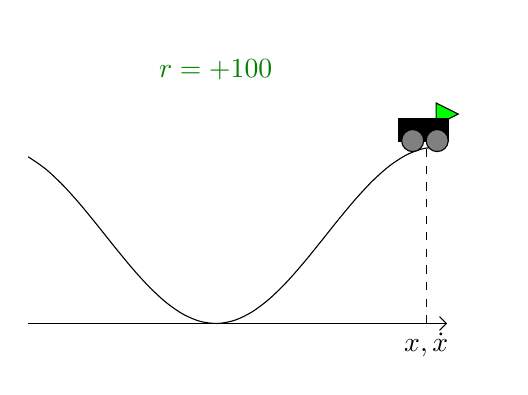
\begin{tikzpicture}[scale=1.4]
%\def\carx{\asdf}
\def\flagheight{4/5}
\def\carlength{0.2}
\def\carx{4.01}

\draw[] (4.05,{\flagheight + 1}) node{\hphantom{asdfasdf}};
\draw[] (2,1.5) node[text=black!50!green,align=center]{$r = +100$};
\draw[] (2,-0.9) node[]{\vphantom{asdf}};

\draw[scale=1,domain=0.3:4.05,smooth,variable=\x] plot ({\x},{\flagheight*cos(90*\x)});

\draw[-,fill=green] (4,\flagheight) -- (4,{\flagheight + 0.4}) -- (4.2,{\flagheight + 0.3}) -- (4,{\flagheight+0.2});



%\def\carx{2.71}
\def\cary{\flagheight*cos(90*\carx)}

%\def\m{\ifthenelse{\equal{\carx}{2}} {100000} {1/(\flagheight*sin(90*\carx))}}

\ifthenelse{\lengthtest{\carx pt < 2 pt}} {\def\fff{-1}} {\def\fff{1}}

\def\m{1/(\flagheight*sin(90*\carx))}
\def\mt{(\flagheight*sin(90*\carx))}
%\def\deltax{(\fff)*sqrt(0.01 / (1 + (\m)*(\m)) )}
\def\deltax{(\fff)*sqrt((0.01*\mt*\mt)/(1 + \mt*\mt))}

\ifthenelse{\lengthtest{\carx pt < 1.85 pt} \OR \lengthtest{\carx pt > 2.15 pt}}{\def\deltay{(\m) * (\deltax)}}{\def\deltay{-0.1}}
%\def\deltay{(\m) * (\deltax)}
\def\carxtwo{\carx - \deltax}
\def\carytwo{\cary - \deltay}


%\ifthenelse{\lengthtest{\carx pt < 1.5 pt} \OR \lengthtest{\carx pt > 2.5 pt}}{\def\carxx{(\carx - \carlength)}}{\def\carxx{(\carx - 2*\carlength  + 0.89*(\carx - 2)^2)}}
%\def\carxx{(\carx - \carlength + -\carlength + 0.5*(\carx - 2)^2)}
\def\carxx{\carx - sqrt((\carlength^2) / (1 + (\mt)^2))}
%\def\carxx{(\carx - \carlength - 0.15*abs(cos(90*\carx)))}
\def\caryy{\flagheight*cos(90*(\carxx))}

%\def\m{\ifthenelse{\equal{\carx}{2}} {100000} {1/(\flagheight*sin(90*\carx))}}

%\def\aaaa{0.15*abs(cos(90*\carx))}

%\setlength{\asdf}{\carx pt - \carlength pt - \aaaa pt }


\FPeval{\asdf}{(\carx - \carlength - 0.15*abs(cos(90*\carx)))}

\ifthenelse{\lengthtest{\asdf pt  < 2 pt }} {\def\ffff{-1}} {\def\ffff{1}}

\def\mm{1/(\flagheight*sin(90*(\carxx)))}
\def\mtt{(\flagheight*sin(90*(\carxx)))}

\def\deltaxx{(\ffff)*sqrt((0.01*(\mtt)*(\mtt))/(1 + (\mtt)*(\mtt)))}

\ifthenelse{\lengthtest{\asdf pt < 1.85 pt} \OR \lengthtest{\asdf pt > 2.15 pt}}{\def\deltayy{(\mm) * (\deltaxx)}}{\def\deltayy{-0.1}}
%\def\deltay{(\m) * (\deltax)}
\def\carxxtwo{\carxx - \deltaxx}
\def\caryytwo{\caryy - \deltayy}





\def\angle{atan((\carxxtwo - \carxtwo) / (\caryytwo - \carytwo)) }

\def\riix{\carxtwo - \carxxtwo}
\def\riiy{\carytwo - \caryytwo}
\def\coeffang{(((\riiy) / (\riix)))}

\def\dddeltax{(sqrt(0.05 / (1 + \coeffang^2)))}
\def\dddeltay{-((\dddeltax) * \coeffang)}

%\draw[-,fill=black,rotate around={{0}:({\carxxtwo},{\caryytwo})}] ({\carxxtwo-0.1},{\caryytwo+0.05}) rectangle({\carxxtwo + sqrt((\carxtwo - \carxxtwo)^2 + (\carytwo - \caryytwo)^2) },{\caryytwo + 0.25});
%\draw[-,fill=black,rotate around={{0}:({\carxxtwo},{\caryytwo})}] ({\carxtwo},{\carytwo}) rectangle({\carxxtwo + sqrt((\carxtwo - \carxxtwo)^2 + (\carytwo - \caryytwo)^2) },{\caryytwo + 0.25});
\draw[line width=0.3cm, black, cap=rect] ({\carxxtwo - \deltaxx}, {\caryytwo - \deltayy}) -- ({\carxtwo - \deltax}, {\caryytwo - \deltayy}); 


\def\deltaxnorm{sqrt((\deltax)^2 + (\deltay)^2)}
\def\deltaxperpnorm{(\deltax)/(\deltaxnorm)}
\def\deltayperpnorm{(\deltay) / (\deltaxnorm)}

\ifthenelse{\lengthtest{\carx pt > 2 pt}}{\def\asdfasdf{2}}{\def\asdfasdf{1}}

%\draw[->,thick,red] ({\carx - 0.2*\deltaxperpnorm}, {\cary - 0.2*\deltayperpnorm}) -- ({\carx - 0.1*\deltaxperpnorm - 0.5*\deltayperpnorm}, {\cary - 0.1*\deltayperpnorm + \asdfasdf* 0.5*\deltaxperpnorm}) node[midway, above]{F};


\draw[-,fill=gray] ({\carxtwo},{\caryytwo}) circle(0.1);
\draw[-,fill=gray] ({\carxxtwo},{\caryytwo}) circle(0.1);

\draw[-angle 90] (0.3,{-\flagheight}) -- (4.1,{-\flagheight});% node[above]{$x$};
\draw[dashed] ({((\carx)+(\carxx))/2},{((\cary) + (\caryy))/2}) -- ({((\carx)+(\carxx))/2}, {-\flagheight}) node[below]{$x, \dot{x}$};
\end{tikzpicture}
}

\end{document}